\section{Architecture 103}

\subsection{Preliminary concept}

\textbf{State - Stateful - Stateless}

\begin{itemize}
	\item State
	variable and instances of a system at a given time
	\item Stateful
	capability of a system to remember preceding event or user insteraction
	e.g., an applicative session of an authenticated user on a Web Site
	\item Stateless
	capability of a system to response always in the same way independently to any sort of previus state
	e.g., a REST API
\end{itemize}

\textbf{Table index*}

\begin{itemize}
	\item An index is an optional structure, associated with a table or table cluster, that sometimes speed data access
	\item By creating an index on one or more caloumns of a table, you gian the ability in some cases to retrive a small set of randomly distributed rows from the table
\end{itemize}

\textbf{Long story short - Lesson Index}

Today we will focus on 3 possibile design patterns
\begin{itemize}
	\item Where and Diff - Change data capture
	How to incrementally retrive data in Big Data and Legacy Apps
	\item Move and Rename - Stateless change data capture
	How not to start from beginning
	\item Wrapper - Lock-in free solutions
	How to mitigate vendor lock-in
\end{itemize}

\subsection{Data Source}

\subsubsection{Data Sources - Log Data}




% \begin{center}
% 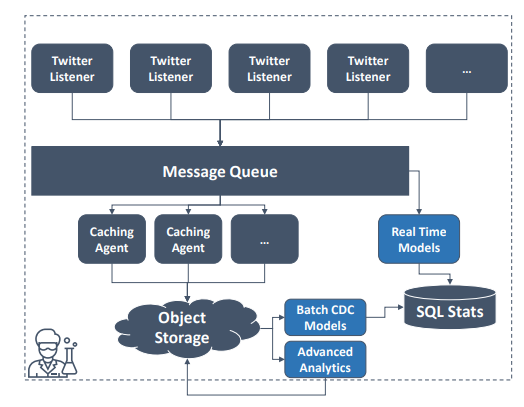
\includegraphics[scale=0.7]{13-architecture-pillars-on-BOC-app}
% \end{center}
